\documentclass{ieeeaccess}
\usepackage{cite}
\usepackage{amsmath,amssymb,amsfonts}
\usepackage{graphicx}
\usepackage{textcomp}

\usepackage{bm}
\makeatletter
\AtBeginDocument{\DeclareMathVersion{bold}
\SetSymbolFont{operators}{bold}{T1}{times}{b}{n}
\SetSymbolFont{NewLetters}{bold}{T1}{times}{b}{it}
\SetMathAlphabet{\mathrm}{bold}{T1}{times}{b}{n}
\SetMathAlphabet{\mathit}{bold}{T1}{times}{b}{it}
\SetMathAlphabet{\mathbf}{bold}{T1}{times}{b}{n}
\SetMathAlphabet{\mathtt}{bold}{OT1}{pcr}{b}{n}
\SetSymbolFont{symbols}{bold}{OMS}{cmsy}{b}{n}
\renewcommand\boldmath{\@nomath\boldmath\mathversion{bold}}}
\makeatother

\graphicspath{{images/}}

\def\BibTeX{{\rm B\kern-.05em{\sc i\kern-.025em b}\kern-.08em
    T\kern-.1667em\lower.7ex\hbox{E}\kern-.125emX}}

\begin{document}
\history{Date of submission May 5, 2026.}
\doi{}

\title{Development of Control Loops for the Fixed-Wing Mode of a Hybrid VTOL Drone}
\author{\uppercase{Kaue Martins de Souza}\authorrefmark{1} and
\uppercase{Neusa Maria Franco}\authorrefmark{1}}

\address[1]{Aeronautics Institute of Technology (ITA), S\~{a}o Jos\'{e} dos Campos, SP 12228-900, Brazil
(e-mail: martinskms@ita.br; neusa@ita.br)}

\tfootnote{This work was developed in the context of the Applied Projects in Electronics graduate course at the Aeronautics Institute of Technology (ITA), in collaboration with the Neusa research group, and builds on the open-source PIPER-1-6 control framework.}

\markboth
{Martins de Souza \MakeLowercase{\textit{et al.}}: Development of Control Loops for the Fixed-Wing Mode of a Hybrid VTOL Drone}
{Martins de Souza \MakeLowercase{\textit{et al.}}: Development of Control Loops for the Fixed-Wing Mode of a Hybrid VTOL Drone}

\corresp{Corresponding author: Kaue Martins de Souza (e-mail: martinskms@ita.br).}


\begin{abstract}
Hybrid Vertical Take-Off and Landing (VTOL) drones combine the hovering capability of multi-rotor systems with the long-range cruise efficiency of fixed-wing aircraft, making them attractive for surveillance, mapping, and last-mile delivery missions. Although the literature is rich in transition and hover control strategies, the design of dedicated longitudinal and lateral-directional control loops for the fixed-wing flight phase of custom hybrid platforms is still under-addressed. This paper presents the design and closed-loop validation of a classical PID-based autopilot for the fixed-wing flight mode of a custom hybrid VTOL drone, leveraging the open-source PIPER-1-6 framework originally validated for the Piper J-3 Cub 1/6 model aircraft. The pipeline spans the 6-DOF nonlinear plant in MATLAB/Simulink, trim and Jacobian-based linearization, and cascaded PID design with stability augmentation systems (SAS) and anti-windup. The control loops are then validated in Software-In-the-Loop (SIL) configuration against the nonlinear model through a campaign of altitude, velocity, heading, and combined step-tracking tests. In every test the autopilot tracks its reference with negligible steady-state error, overshoot below $15\%$, and unsaturated control effort (surface deflections at or below $4.5^\circ$ of the $\pm 25^\circ$ travel), and the nonlinear response is found to be more damped than the linear design model owing to the quadratic aerodynamic terms and the energy-to-speed coupling. The results confirm that the Piper J-3 Cub cascaded-PID framework transfers to the hybrid VTOL platform with only re-tuned gains, and that classical cascaded PID remains a robust, interpretable, and low-cost solution for the cruise envelope considered.
\end{abstract}

\begin{keywords}
Autopilot, fixed-wing flight, flight control system, hybrid VTOL drone, linearization, MATLAB/Simulink, PID control, software-in-the-loop, stability augmentation system, unmanned aerial vehicle.
\end{keywords}

\titlepgskip=-21pt

\maketitle

\section{Introduction}
\label{sec:introduction}

\subsection{Importance of the Topic}

\PARstart{U}{nmanned} Aerial Vehicles (UAVs) were originally developed for military reconnaissance and strike missions, but their use has rapidly expanded to civil and academic applications, including search-and-rescue, environmental monitoring, precision agriculture, last-mile delivery, and aerial cinematography \cite{beard2005autonomous,marshall2016introduction}. The growing availability of low-cost embedded electronics, brushless motors, lithium-polymer batteries, and microelectromechanical (MEMS) inertial sensors has enabled the proliferation of small UAVs, while at the same time raising the demand for more robust and precise autonomous flight control systems that minimize human intervention and operational risk \cite{garcia2010multi,valavanis2015future}.

Among the various airframe configurations, hybrid Vertical Take-Off and Landing (VTOL) drones have emerged as a particularly attractive class of platforms. They combine the static-thrust capability of multi-rotor systems --- which allows them to take off, hover, and land vertically without the need for runways --- with the higher cruise efficiency and longer endurance of fixed-wing aircraft, which rely on aerodynamic lift instead of continuous rotor thrust \cite{saeed2018survey,ducard2021review}. This dual nature, however, comes at the cost of a more complex flight envelope: hybrid VTOLs operate in three distinct modes --- hover, transition, and cruise --- each one with its own dynamics, actuator allocation, and control objectives \cite{ducard2021review}.

\begin{figure}[!htbp]
    \centerline{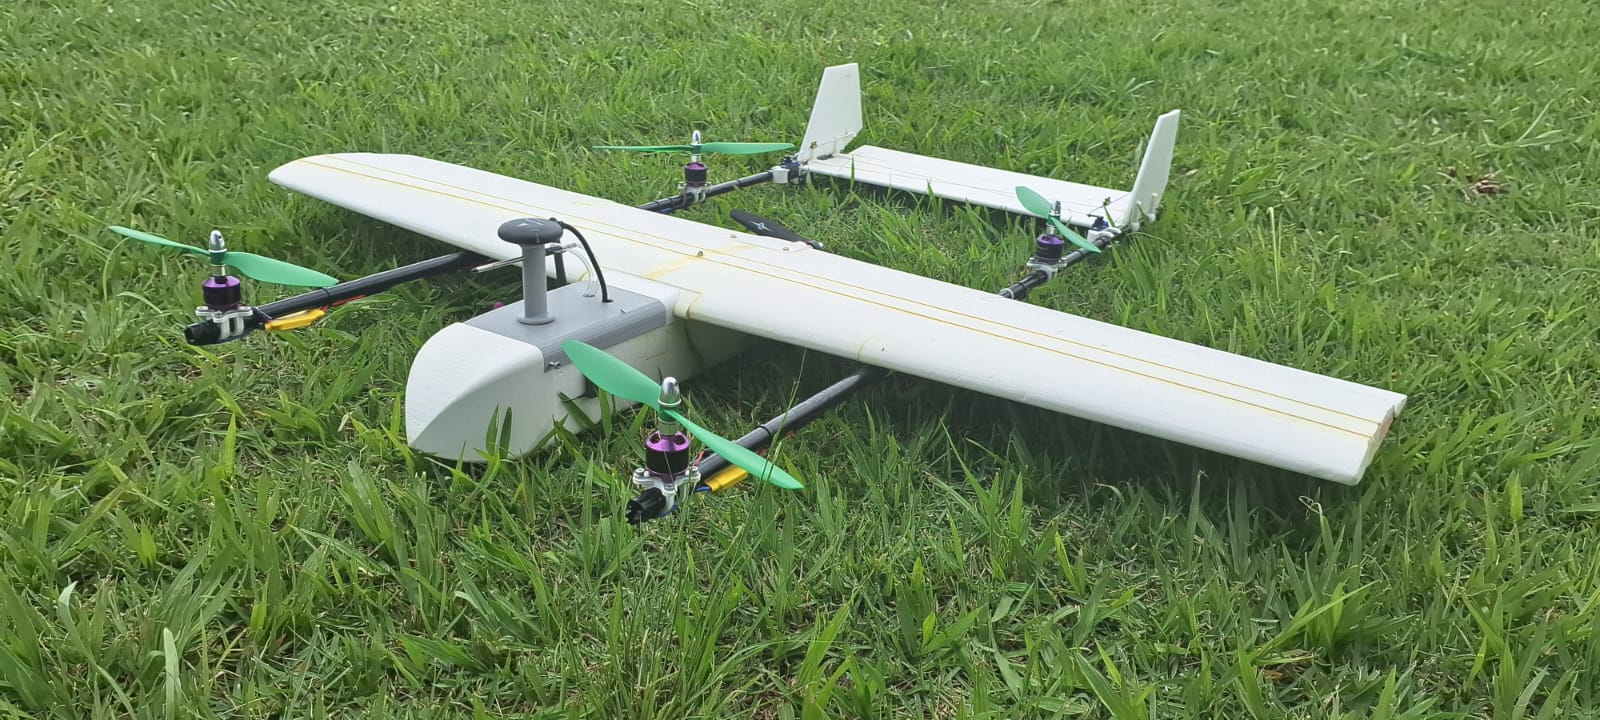
\includegraphics[width=0.85\columnwidth]{fig_drone.jpg}}
    \caption{Custom hybrid VTOL drone developed by the Neusa research group at the Aeronautics Institute of Technology (ITA), used as the target platform for the fixed-wing autopilot designed in this work.}
    \label{fig:drone}
\end{figure}

The development of reliable autopilots for hybrid platforms is therefore a non-trivial task. Although the hover and transition phases have received the larger part of the research effort, the fixed-wing cruise phase remains crucial for mission performance, since it is during cruise that the platform covers the bulk of the operational distance. In cruise, aerodynamic modeling and the careful tuning of the longitudinal and lateral-directional control loops are essential to guarantee stability, gust rejection, and tracking accuracy \cite{levin2019real,chao2010autopilots}.

\subsection{What is Known (State of the Art)}

In the open-source ecosystem, the PX4 autopilot stack running on Pixhawk hardware has become a widely adopted reference for fixed-wing and hybrid UAV flight control, both in industry and in academic research \cite{meier2015px4,px4dev2025}. Its fixed-wing module is built around the Total Energy Control System (TECS), an energy-based scheme in which throttle commands the total energy and pitch its distribution between altitude and airspeed, complemented by a cascaded attitude/rate controller with airspeed scaling and coordinated-turn compensation. While elegant from a multivariable standpoint, TECS requires accurate aerodynamic and propulsion models and careful feed-forward integration --- assets that are often unavailable for custom academic platforms.

A more accessible alternative --- and the one followed in this work --- is the classical autopilot architecture introduced by Stevens and Lewis \cite{stevens2016aircraft} and Nelson \cite{nelson1998flight}, in which the longitudinal and lateral-directional dynamics are decoupled around a trim point and addressed by a hierarchy of cascaded loops: an inner stability augmentation system (SAS) that uses angular-rate feedback to damp the natural modes, and outer attitude/altitude/heading loops with PID compensators tuned via root-locus or interactive tuning tools. Although less elegant than energy-based formulations, this approach is well documented, fast to tune, and has been successfully applied to a number of small fixed-wing aircraft \cite{beard2012small,cetin2012continuous,du2011development}.

In particular, two prior projects developed at the Aeronautics Institute of Technology (ITA) form the technical foundation of the present work. The Pegasus AutoPilot, presented by Santos \cite{santos2018projeto}, proposed a complete classical autopilot for the Piper J-3 Cub 1/4 model aircraft, including a 6-DOF nonlinear plant and longitudinal and lateral-directional control loops. The architecture of the central processing unit of the Pegasus platform was further detailed by Bittar \cite{bittar2012arquitetura}. Building on these works, the open-source PIPER-1-6 project \cite{martins2025piper} re-implemented and extended the Pegasus framework for the Piper J-3 Cub 1/6, providing a fully reproducible MATLAB/Simulink toolchain that includes parameter loading, trim computation via \texttt{fmincon}, model linearization, PID tuning, and waypoint guidance.

\subsection{What is Unknown (Research Gap)}

Despite this consolidated body of work, several gaps remain when one tries to transfer those control loops to a hybrid VTOL platform operating in fixed-wing mode. First, regarding \textit{model transferability}, control loops designed for conventional fixed-wing UAVs (e.g., the Piper J-3 Cub 1/6) have not been systematically adapted and validated for hybrid VTOL platforms operating in fixed-wing mode. Second, in terms of \textit{aerodynamic differences}, hybrid drones present distinct aerodynamic characteristics due to motor placement, propeller interactions, and airframe geometry, requiring revalidation of the stability derivatives and the control gains \cite{saeed2018survey,theys2016influence}. Third, considering \textit{integrated fixed-wing control}, most hybrid VTOL research focuses on transition and hover; fewer studies address the design of dedicated longitudinal and lateral-directional control loops optimized for the cruise phase of custom hybrid platforms \cite{ducard2021review}. Finally, on the methodological side, there is a need for accessible \textit{simulation-first} pipelines that enable iterative control design before committing to costly and risky flight campaigns, especially for academic groups that lack dedicated wind-tunnel or telemetry facilities \cite{filho2019aerodynamic,bristeau2009role}.

\subsection{Research Objective}

The main objective of this work is to design, implement, and validate the longitudinal and lateral-directional control loops for the fixed-wing flight mode of a custom hybrid VTOL drone, leveraging the control framework developed in the PIPER-1-6 project. The specific objectives are:
\begin{enumerate}
    \item to characterize the aerodynamic model of the hybrid drone in fixed-wing configuration using Vortex Lattice methods (XFLR5/AVL);
    \item to obtain the linearized state-space representation of the aircraft dynamics at the cruise trim condition;
    \item to design PID-based control loops for pitch, airspeed, and altitude (longitudinal channel) and for roll and yaw (lateral-directional channel) using classical control techniques;
    \item to validate the closed-loop system through Software-In-the-Loop (SIL) simulation in MATLAB/Simulink with the 6-DOF nonlinear model;
    \item to evaluate the closed-loop controller performance through step-tracking tests on the nonlinear plant, and to relate the outcome to the Piper J-3 Cub 1/6 baseline framework.
\end{enumerate}

\subsection{Approach Overview}

Starting from the PIPER-1-6 open-source autopilot \cite{martins2025piper}, the proven Piper J-3 Cub 1/6 framework is adapted to the hybrid platform through a five-step pipeline: (1) aerodynamic characterization; (2) assembly of the 6-DOF nonlinear model in MATLAB/Simulink; (3) trim and linearization at the cruise condition; (4) design of the cascaded longitudinal and lateral-directional loops; and (5) closed-loop Software-In-the-Loop (SIL) validation against the nonlinear plant. The strategy is a classical PID autopilot with an inner rate-feedback SAS and an outer attitude/altitude/heading layer, tuned on the linearized plant. Each of these steps is detailed in Section~\ref{sec:methods}.

\subsection{Main Contributions}

The main contributions of this work are the following:
\begin{enumerate}
    \item an \textit{adapted control framework} that systematically transfers the Piper J-3 Cub 1/6 autopilot loops to a custom hybrid VTOL drone operating in fixed-wing mode, illustrating the portability of classical control techniques across different airframes;
    \item a \textit{hybrid-drone aerodynamic and dynamic model}, including stability derivatives and a validated 6-DOF simulation environment in MATLAB/Simulink for the fixed-wing configuration;
    \item an \textit{open-source extension} of the PIPER-1-6 project to support hybrid VTOL platforms, contributing a reusable simulation and control-design framework to the academic community.
\end{enumerate}

The remainder of this paper is organized as follows. Section~\ref{sec:methods} describes the methodology adopted in the project, including the aerodynamic and 6-DOF mathematical models, the trim and linearization procedure, the control architecture for both flight axes, and the simulation framework. Section~\ref{sec:results} presents the objective closed-loop validation results, Section~\ref{sec:discussion} interprets them, compares the work with prior art, and states its limitations and future directions, and Section~\ref{sec:conclusion} draws the final conclusions.

\section{Materials and Methods}
\label{sec:methods}

\subsection{Target Aircraft and Aerodynamic Model}

The platform considered in this work is a custom hybrid VTOL drone developed by the Neusa research group at ITA (see Fig.~\ref{fig:drone}). The aircraft is composed of a fixed-wing fuselage carrying four lift rotors mounted on tail booms for the VTOL phase and a single tractor propeller for forward thrust. In fixed-wing mode, the lift rotors are switched off and the aircraft behaves as a conventional rear-elevator/aileron/rudder airplane.

The stability and control derivatives of the hybrid drone in cruise configuration were obtained by another member of the project group through Vortex Lattice methods (XFLR5/AVL). Because the present work focuses on control design, the aerodynamic model was treated as an external input. The model comprises the dimensionless force and moment coefficients $C_L$, $C_D$, $C_m$, $C_Y$, $C_l$, $C_n$ and their partial derivatives with respect to the angle of attack $\alpha$, the sideslip angle $\beta$, the body-axis rates $p$, $q$, $r$, and the control deflections $\delta_e$, $\delta_a$, $\delta_r$ --- the linear sensitivities that close the rigid-body equations of motion. Together with the reference geometry (wing area $S$, mean aerodynamic chord $\bar{c}$, span $b$) and the air density $\rho$, they yield the dynamic pressure $q_\infty = \tfrac{1}{2}\rho V_T^2$ and the aerodynamic forces and moments at every integration step.

For comparison, the same control architecture was also instantiated for the Piper J-3 Cub 1/6, whose aerodynamic data come pre-validated from the PIPER-1-6 repository \cite{martins2025piper}. The Piper J-3 Cub 1/6 is a 1/6-scale radio-controlled model of the original Piper J-3 Cub and serves as the prior-work reference for the control framework, while the hybrid drone itself was trimmed and validated in this work at its own cruise condition ($V_e = 12$~m/s, $h_e = 600$~m). Both aircraft were described by a 12-state vector,
\begin{equation}
\mathbf{x} = \left[ u, v, w, p, q, r, \phi, \theta, \psi, x_N, x_E, x_D \right]^\top,
\label{eq:state}
\end{equation}
and by four control inputs,
\begin{equation}
\mathbf{u} = \left[ \delta_T, \delta_e, \delta_a, \delta_r \right]^\top,
\label{eq:inputs}
\end{equation}
representing throttle, elevator, aileron and rudder commands, respectively. A bootstrap script in MATLAB loads the full set of geometric and inertial parameters of both airframes (wing reference area, mean aerodynamic chord, span, mass, and moments of inertia) into the workspace, ensuring that every Simulink model in the toolchain is exercised against the same aircraft definition.

\subsection{6-DOF Nonlinear Plant in MATLAB/Simulink}

The aircraft dynamics were described by the standard six-degree-of-freedom rigid-body equations of motion \cite{stevens2016aircraft,nelson1998flight}:
\begin{equation}
m\,\dot{\mathbf{v}} = \mathbf{F}_\text{aero} + \mathbf{F}_\text{grav} + \mathbf{F}_\text{prop},
\label{eq:force}
\end{equation}
\begin{equation}
\mathbf{I}\,\dot{\boldsymbol{\omega}} + \boldsymbol{\omega}\times(\mathbf{I}\,\boldsymbol{\omega}) = \mathbf{M}_\text{aero} + \mathbf{M}_\text{prop},
\label{eq:moment}
\end{equation}
where $\mathbf{v} = [u, v, w]^\top$ is the body-axis linear velocity vector, $\boldsymbol{\omega} = [p, q, r]^\top$ is the body-axis angular velocity, $m$ is the aircraft mass, and $\mathbf{I}$ is the inertia tensor. The aerodynamic forces and moments $\mathbf{F}_\text{aero}$, $\mathbf{M}_\text{aero}$ were computed from the stability derivatives, the dynamic pressure, and the control deflections, while the propulsion forces and moments $\mathbf{F}_\text{prop}$, $\mathbf{M}_\text{prop}$ were obtained from a static propeller model fed by the throttle command. Euler angle kinematics and NED-frame position equations closed the model.

In MATLAB/Simulink, the entire 6-DOF nonlinear plant was implemented as a single compiled C-MEX S-function with twelve internal states, four control inputs, and twenty-one outputs (the twelve states plus airspeed $V_T$, angle of attack $\alpha$, sideslip $\beta$, altitude $h$, body-axis accelerations, and additional monitoring channels). The same S-function was reused as the reference plant by the closed-loop control-validation model employed in this work, guaranteeing that every test was run against an identical aircraft model; a mission-level model driven by a Line-Of-Sight waypoint-guidance law is part of ongoing work. The development environment was MATLAB/Simulink R2024a or later (tested up to R2025b), with the Optimization Toolbox required for the trim procedure described in Section~\ref{sec:trim}. All Simulink models were exercised with the fixed-step fourth-order Runge--Kutta solver \texttt{ode4} at a sampling time of $T_s = 0.01$~s, with a default simulation horizon of $60$~s for the step-response tests.

\subsection{Trim Condition and Linearization}
\label{sec:trim}

The trim, or equilibrium, condition is the steady-state flight regime in which all body-axis accelerations vanish, i.e.,
\begin{equation}
\dot{\mathbf{x}} = f(\mathbf{x}_0, \mathbf{u}_0) = \mathbf{0}.
\label{eq:trim}
\end{equation}
For straight-and-level cruise flight, this corresponds to constant airspeed $V_T$ (thrust equals drag), constant altitude $h$ (lift equals weight), wings level ($\phi_0 = 0$), and zero angular rates ($p_0 = q_0 = r_0 = 0$).

Because the nonlinear equations of motion contain trigonometric and quadratic terms in the aerodynamic coefficients, the trim problem does not admit a closed-form solution and must be solved numerically. The PIPER-1-6 toolchain casts the problem as a constrained nonlinear optimization, solved by MATLAB's \texttt{fmincon} from the Optimization Toolbox. A trim-candidate vector was used to set the initial states and control inputs of the Simulink model; the model was then evaluated for an instant; the resulting accelerations were extracted; and the cost function
\begin{equation}
J(\mathbf{x}, \mathbf{u}) = \left\| \dot{\mathbf{x}} \right\|^2
\label{eq:trim-cost}
\end{equation}
was minimized iteratively with physically plausible bounds on the decision variables (throttle within $[0, 1]$ and the three control surfaces within $\pm 25^\circ$). Convergence was declared whenever $J$ fell below a tolerance of $10^{-6}$.

Once the trim point $(\mathbf{x}_0, \mathbf{u}_0)$ is known, a small-perturbation linearization yields the state-space model
\begin{equation}
\Delta\dot{\mathbf{x}} = \mathbf{A}\,\Delta\mathbf{x} + \mathbf{B}\,\Delta\mathbf{u}, \quad \Delta\mathbf{y} = \mathbf{C}\,\Delta\mathbf{x} + \mathbf{D}\,\Delta\mathbf{u},
\label{eq:linear}
\end{equation}
with $\mathbf{A}$ and $\mathbf{B}$ obtained by numerically evaluating the Jacobians of $f(\mathbf{x}, \mathbf{u})$ around $(\mathbf{x}_0, \mathbf{u}_0)$. Three independent linearization methods were compared in the PIPER-1-6 project --- a hand-coded script following Nelson's book \cite{nelson1998flight}, an analytic implementation, and MATLAB's built-in \texttt{linearize} command, which numerically perturbs the Simulink model around the operating point --- and the smallest RMSE against the nonlinear plant was obtained, respectively, by \texttt{linearize} for the longitudinal channel and by the analytical script for the lateral-directional channel. The system naturally decoupled into two five-state subsystems:
\begin{equation}
\mathbf{x}_\text{long} = \left[ u, w, q, \theta, h \right]^\top,\quad \mathbf{u}_\text{long} = \left[ \delta_T, \delta_e \right]^\top,
\label{eq:longstate}
\end{equation}
\begin{equation}
\mathbf{x}_\text{lat} = \left[ v, p, r, \phi, \psi \right]^\top,\quad \mathbf{u}_\text{lat} = \left[ \delta_a, \delta_r \right]^\top.
\label{eq:latstate}
\end{equation}
The corresponding eigenvalues revealed the four classical modes of the airframe --- short-period and phugoid in the longitudinal channel, dutch-roll, spiral, and pure-roll in the lateral channel.

\subsection{Longitudinal Control Loops}
\label{sec:longctrl}

The longitudinal autopilot follows the cascaded structure proposed by Stevens and Lewis \cite{stevens2016aircraft} and refined by Santos \cite{santos2018projeto}. Three loops act in parallel to control airspeed, pitch attitude, and altitude.

\begin{figure}[!htbp]
    \centerline{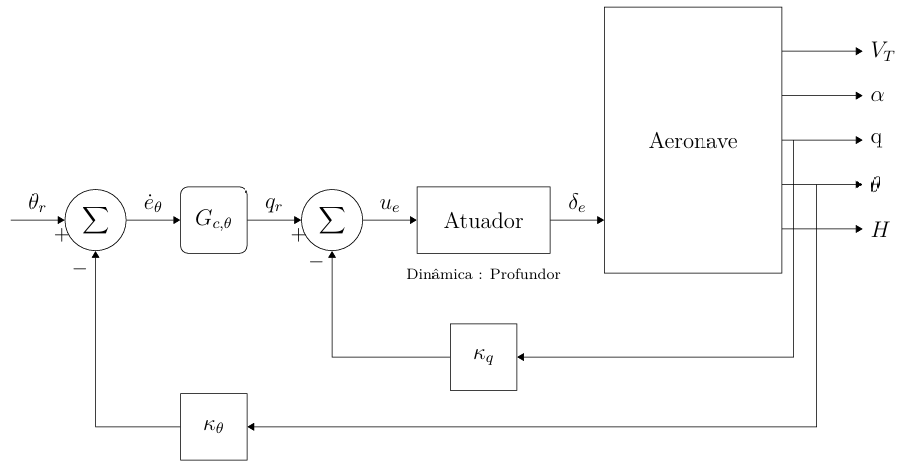
\includegraphics[width=\columnwidth]{fig_pitch.png}}
    \caption{Pitch attitude autopilot with stability augmentation system (SAS), adapted from Santos \cite{santos2018projeto}.}
    \label{fig:pitch}
\end{figure}

\textit{1) Pitch attitude with SAS:} the innermost loop tracks a pitch reference $\theta_\text{ref}$. The pitch rate $q$ is fed back through a proportional gain $K_q = 0.0524$ (root-locus tuned to obtain a damping ratio of about $0.70$ on the short-period mode), forming a stability augmentation system that damps the natural short-period oscillation. Around this SAS, a PI compensator with $K_p = 0.4007$, $K_i = 0.3918$, $K_d = 0$ and a derivative-filter coefficient $N = 100$ closes the outer pitch loop ($\omega_c = 2.0$~rad/s, phase margin $65^\circ$). The elevator deflection $\delta_e$ is saturated at $\pm 25^\circ$ ($\pm 0.4363$~rad) and the integrator is protected with a clamping anti-windup scheme.

\begin{figure}[!htbp]
    \centerline{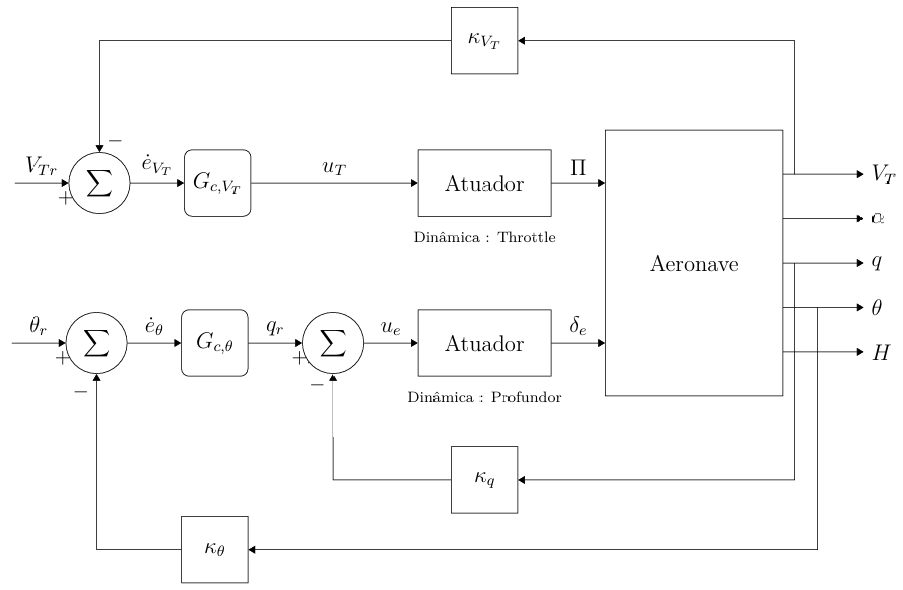
\includegraphics[width=\columnwidth]{fig_velocity_block.png}}
    \caption{Velocity autopilot: a PID throttle loop runs in parallel with the pitch attitude loop, attenuating the speed loss caused by climb maneuvers.}
    \label{fig:velocity}
\end{figure}

\textit{2) Velocity autopilot:} a parallel PI compensator with $K_p = 0.2899$, $K_i = 0.0870$, $K_d = 0$, $N = 100$ ($\omega_c = 0.8$~rad/s), acting on the airspeed error $e_V = V_{T,\text{ref}} - V_T$, drives the throttle command $\delta_T$. The throttle is saturated to the unit interval $[0, 1]$ and the integrator is again clamped. The simultaneous action of the pitch loop on the elevator and the velocity loop on the throttle attenuates the speed losses naturally caused by climbing maneuvers, when only the elevator is commanded.

\begin{figure}[!htbp]
    \centerline{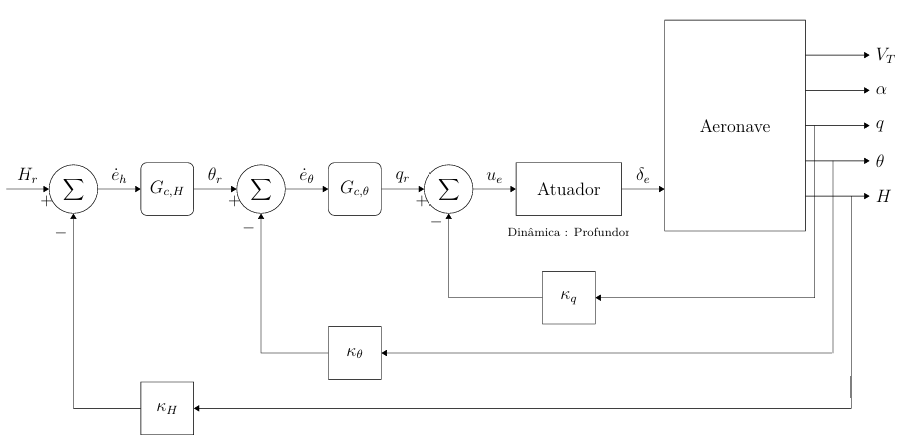
\includegraphics[width=\columnwidth]{fig_altitude_block.png}}
    \caption{Altitude hold autopilot: an outer PID generates the pitch reference $\theta_\text{ref}$ tracked by the inner pitch attitude loop.}
    \label{fig:altitude}
\end{figure}

\textit{3) Altitude hold:} an outer PI compensator with $K_p = 0.02875$, $K_i = 0.00259$, $K_d = 0$, $N = 100$ ($\omega_c = 0.35$~rad/s, phase margin $55^\circ$, gain margin $26$~dB) converts the altitude error $e_h = h_\text{ref} - h$ into a pitch reference $\theta_\text{ref}$ that is then tracked by the pitch attitude loop. The output of the altitude compensator is clamped to $\pm 0.1745$~rad ($\pm 10^\circ$) to bound the commanded pitch and keep the angle of attack away from stall (the trim $\alpha \approx 14.4^\circ$, and no stall model is included in the plant).

\subsection{Lateral-Directional Control Loops}

\begin{figure*}[!htbp]
    \centerline{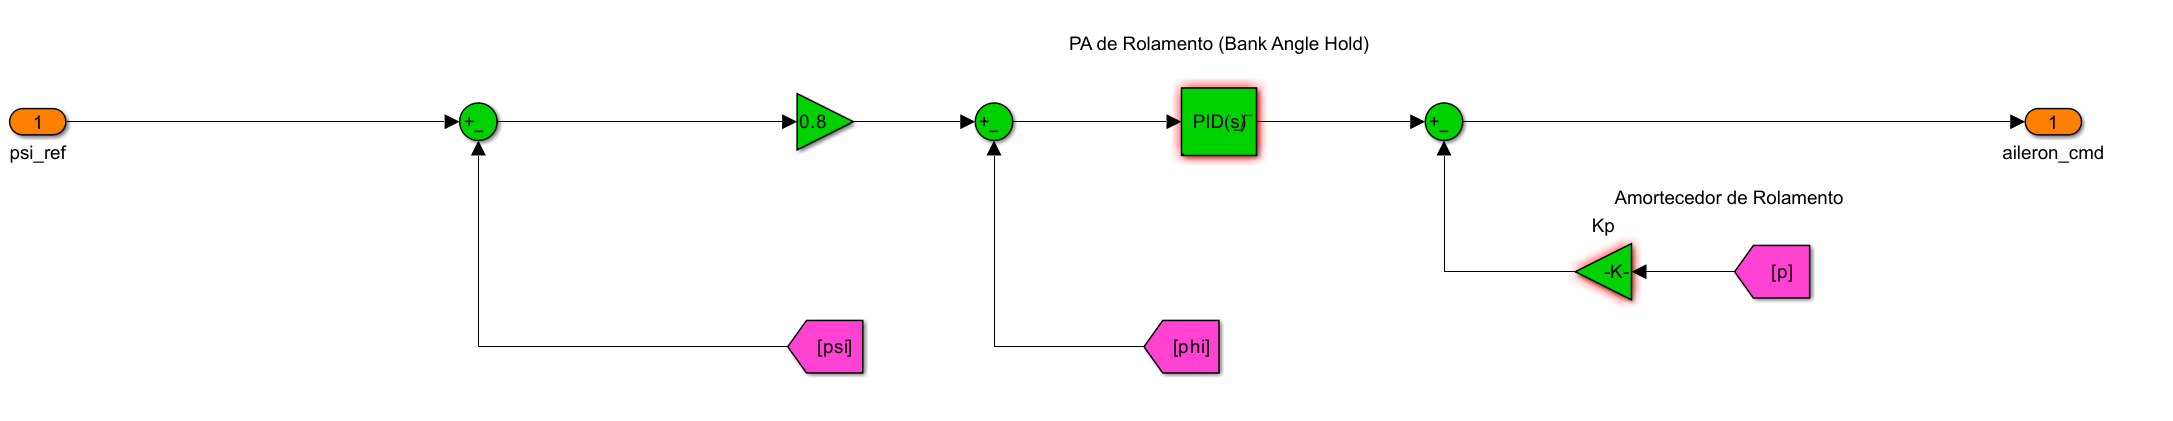
\includegraphics[width=0.85\textwidth]{fig_bank.png}}
    \caption{Bank angle hold autopilot with roll SAS and heading-select feed-forward (PIPER-1-6 Simulink model).}
    \label{fig:bank}
\end{figure*}

\textit{1) Bank angle hold:} heading commands are converted into a bank-angle reference through a heading-select gain $K_\text{heading} = u_e/(g\,\tau_\psi) = 0.1975$ (with a desired heading time constant $\tau_\psi = 6$~s), exploiting the coordinated-turn approximation
\begin{equation}
\phi \approx \frac{\dot{\psi}\,u_0}{g}.
\label{eq:cordturn}
\end{equation}
The roll attitude is then tracked by a PI compensator with $K_p = -0.2831$, $K_i = -0.2716$, $K_d = 0$, $N = 100$ ($\omega_c = 2.0$~rad/s, phase margin $65^\circ$), whose output drives the aileron channel. The gains are \emph{negative} because the drone's roll-control derivative is negative ($C_{l_{\delta a}} < 0$), so that a negative gain preserves negative feedback. No roll-rate SAS gain is required ($K_{p,\text{sas}} = 0$): the bare-airframe roll mode already meets Level-1 handling with margin. The aileron is saturated at $\pm 25^\circ$, and back-calculation anti-windup is used.

\begin{figure}[!htbp]
    \centerline{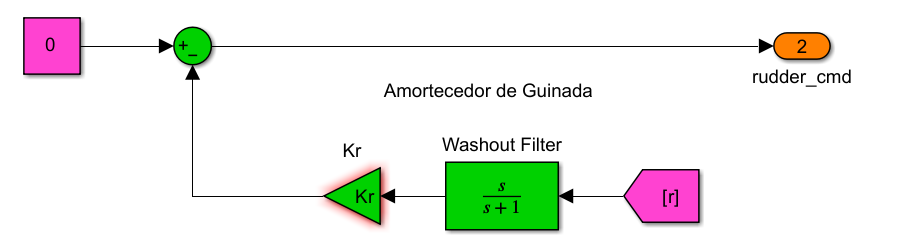
\includegraphics[width=\columnwidth]{fig_yaw_damper.png}}
    \caption{Yaw damper with washout filter on yaw rate $r$, used to damp dutch-roll oscillations without opposing steady-state coordinated turns.}
    \label{fig:yawdamper}
\end{figure}

\textit{2) Yaw damper:} dutch-roll oscillations are damped by feeding the yaw rate $r$ through a first-order washout filter,
\begin{equation}
G_w(s) = \frac{\tau_w\,s}{1 + \tau_w\,s},
\label{eq:washout}
\end{equation}
with $\tau_w = 1$~s, multiplied by a static gain $K_r = 0.1481$ (tuned for a dutch-roll damping ratio of about $0.707$), and applied to the rudder channel. The washout filter passes only the transient $r$ variations, preventing the rudder from biasing the steady-state coordinated turn. The rudder is saturated at $\pm 25^\circ$. This damper attenuates the dutch-roll mode but does not perform turn coordination, which would require an additional sideslip feedback loop ($\beta \to \delta_r$).

\subsection{Simulation and Validation Framework}

The control design followed a structured Software-In-the-Loop (SIL) validation pipeline with two levels of increasing fidelity: (i) loop shaping on the linearized plant, where the PI compensators were tuned sequentially (inner loop first) with MATLAB's \texttt{pidtune} to meet the bandwidth and stability-margin targets reported in Section~\ref{sec:longctrl}; and (ii) closed-loop SIL on the nonlinear Simulink plant under step references around the cruise trim, in order to assess the robustness of each loop to the residual nonlinearities of the model. Any inconsistency between the two levels can thus be detected and isolated as soon as it appears.

The performance of each loop was then assessed from the SIL time histories through the step-response indicators detailed in Section~\ref{sec:results} --- rise time, percent overshoot, settling time within a $\pm 2\%$ band, steady-state error, and peak actuator deflection. Because the simulations are deterministic and noise-free, each scenario was executed once and only these deterministic time-series indicators were used; no statistical (e.g., Monte-Carlo) dispersion analysis was performed at this stage.

\section{Results}
\label{sec:results}

This section reports the closed-loop validation of the cascaded PID autopilot designed for the hybrid VTOL drone. All results were obtained in closed loop on the nonlinear 6-DOF model, with the controller gains held fixed across every test. Following the guidance of Section~\ref{sec:methods}, the findings are reported here objectively; their interpretation, the comparison with prior work, and the study limitations are deferred to Section~\ref{sec:discussion}.

\subsection{Simulation Setup and Evaluation Criteria}

The plant is the nonlinear 6-DOF S-function described in Section~\ref{sec:methods}, closed by the cascaded PID autopilot with fixed gains. The aircraft was trimmed in straight-and-level cruise at $V_e = 12$~m/s and $h_e = 600$~m, which corresponds to a trim throttle of $\delta_T \approx 0.25$; the control surfaces are limited to $\pm 25^\circ$ and the throttle to the unit interval $[0,1]$. Four step-tracking scenarios were exercised (Table~\ref{tab:scenarios}): three of them isolate a single autopilot loop (altitude, velocity, heading), while the fourth commands altitude and heading simultaneously to excite the longitudinal and lateral-directional axes at once.

\begin{table}[!htbp]
\caption{Closed-loop step-tracking test scenarios.}
\label{tab:scenarios}
\centering
\begin{tabular}{lll}
\hline
\textbf{Scenario} & \textbf{Reference step} & \textbf{Applied} \\
\hline
Altitude hold & $+50$~m ($600 \to 650$~m) & $t = 0$ \\
Velocity hold & $+6$~m/s ($12 \to 18$~m/s) & $t = 0$ \\
Heading hold  & $+20^\circ$ & $t = 5$~s \\
Combined      & $+30$~m \& $+15^\circ$ & $t = 5$~s \\
\hline
\end{tabular}
\end{table}

The performance of each loop was quantified with the standard step-response indicators computed by MATLAB's \texttt{stepinfo}: rise time (time to first reach the reference), percent overshoot (peak excursion beyond the reference), settling time (entry into the $\pm 2\%$ band), and steady-state error (residual at regime). The peak control effort of each actuator was also recorded and compared against the physical limits.

\subsection{Scenario 1: Altitude Hold ($+50$~m Step)}

The altitude loop drove $h$ from $600$~m to the $+50$~m reference (Fig.~\ref{fig:s1_alt}). The outer loop generated a pitch command of up to about $20^\circ$, which the inner pitch loop tracked closely, and the resulting elevator activity peaked at $4.5^\circ$ --- well within the $\pm 25^\circ$ limit (Fig.~\ref{fig:s1_act}). The measured indicators were a rise time of $12.9$~s, an overshoot of $8.7\%$, a settling time of $32.7$~s, and a steady-state error of $0.04$~m.

\begin{figure}[!htbp]
\centerline{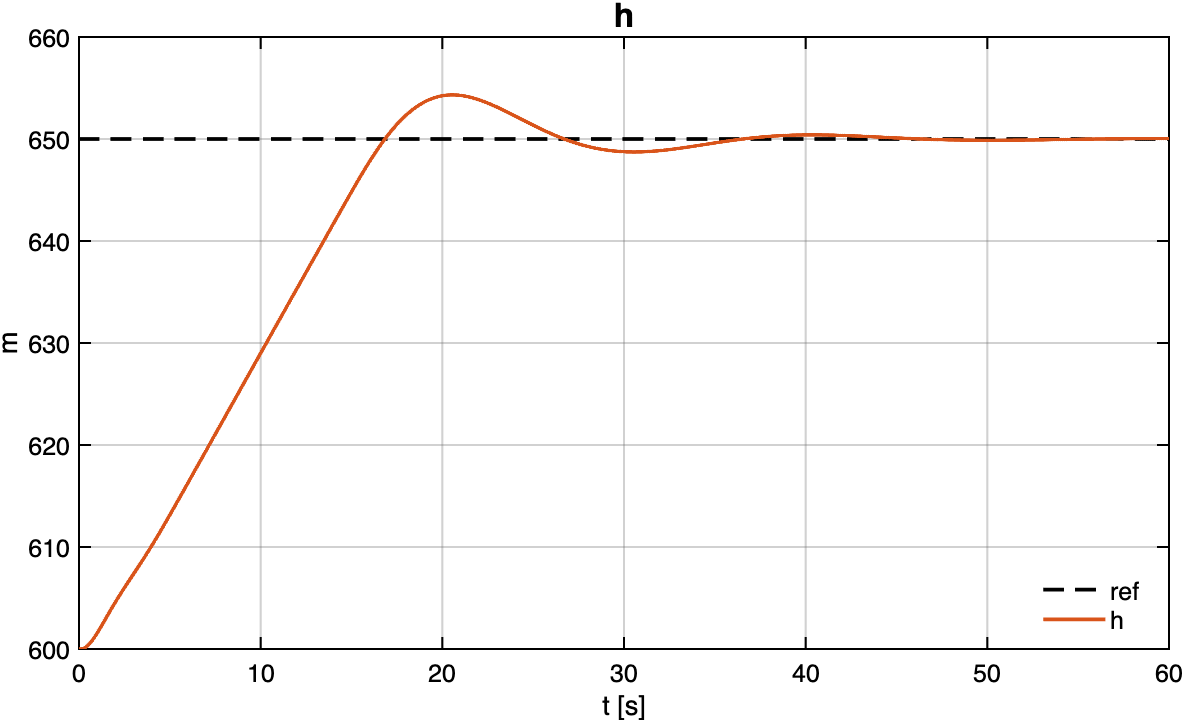
\includegraphics[width=\columnwidth]{fig_s1_alt.png}}
\caption{Scenario 1 --- altitude $h(t)$ tracking the $+50$~m step (solid) against the reference (dashed).}
\label{fig:s1_alt}
\end{figure}

\begin{figure}[!htbp]
\centerline{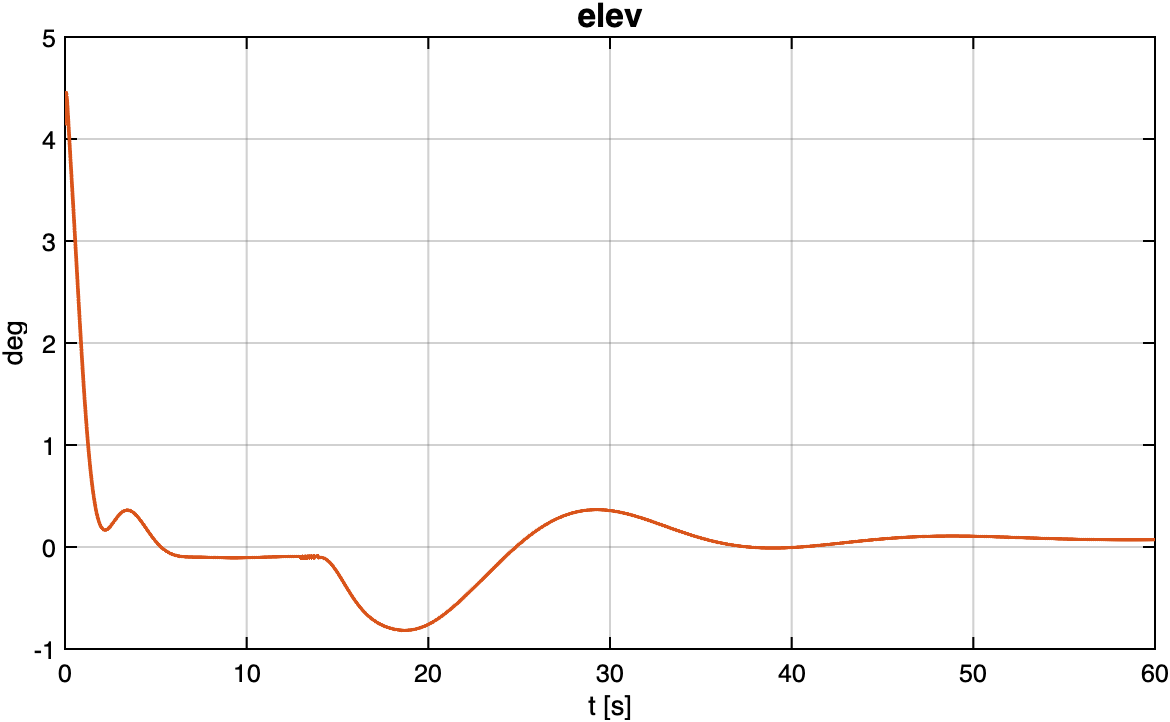
\includegraphics[width=\columnwidth]{fig_s1_elev.png}}
\caption{Scenario 1 --- elevator deflection (deg), peaking at $4.5^\circ$.}
\label{fig:s1_act}
\end{figure}

\subsection{Scenario 2: Velocity Hold ($+6$~m/s Step)}

The throttle rose to $0.76$ to accelerate the aircraft from $12$ to $18$~m/s (Figs.~\ref{fig:s2_vel} and~\ref{fig:s2_thr}), while the altitude stayed within $2.2$~m of $600$~m throughout the maneuver. The velocity response had a rise time of $2.5$~s, an overshoot of $8.0\%$, a settling time of $8.1$~s, and a negligible steady-state error.

\begin{figure}[!htbp]
\centerline{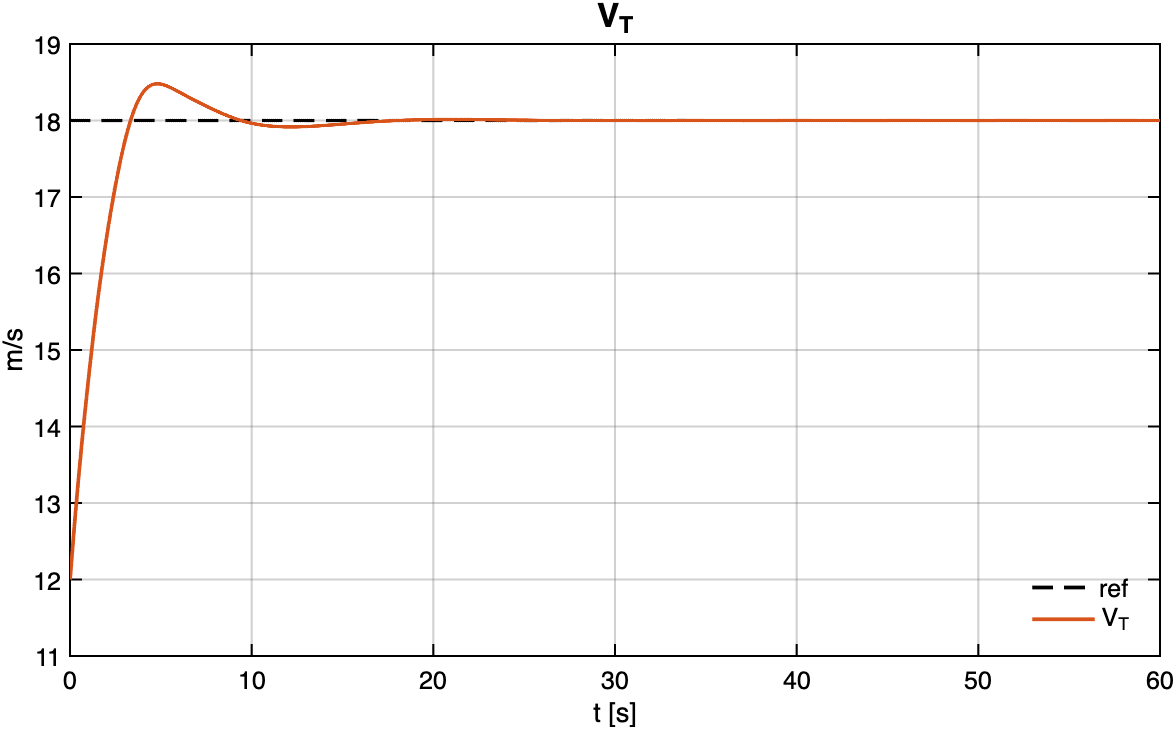
\includegraphics[width=\columnwidth]{fig_s2_vel.png}}
\caption{Scenario 2 --- airspeed $V_T(t)$ tracking the $+6$~m/s step.}
\label{fig:s2_vel}
\end{figure}

\begin{figure}[!htbp]
\centerline{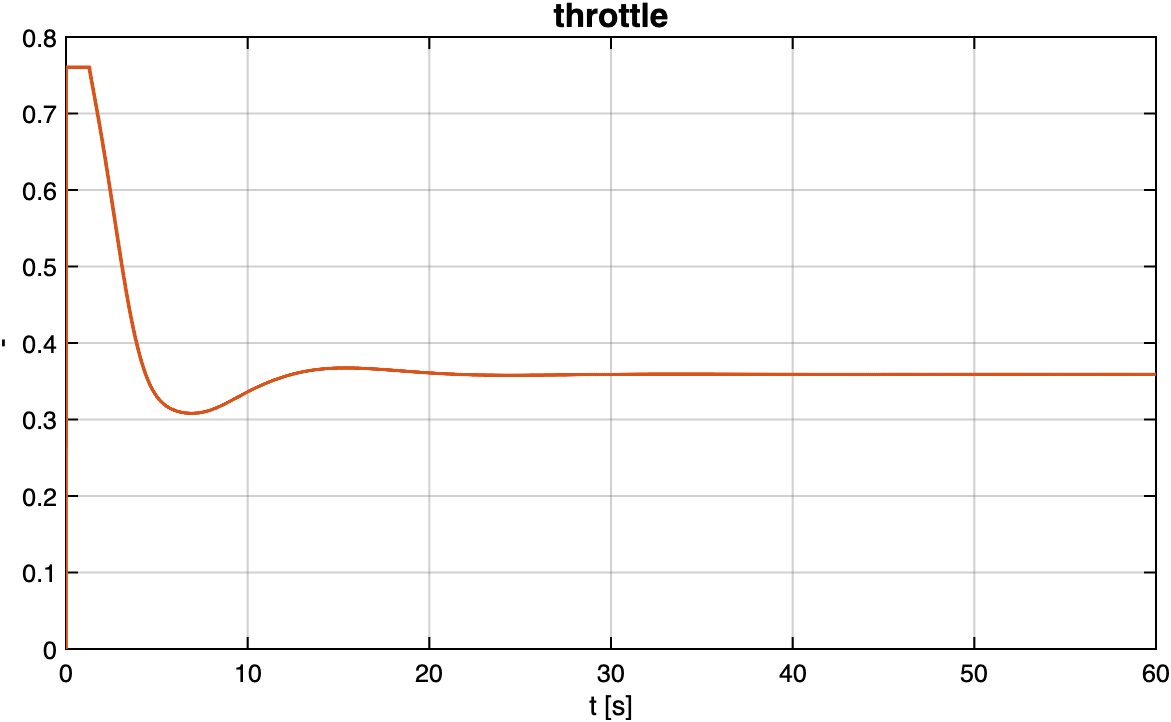
\includegraphics[width=\columnwidth]{fig_s2_thr.png}}
\caption{Scenario 2 --- throttle command ($0$--$1$), peaking at $0.76$.}
\label{fig:s2_thr}
\end{figure}

\subsection{Scenario 3: Heading Hold ($+20^\circ$ Step)}

The heading command ($+20^\circ$ applied at $t = 5$~s, Fig.~\ref{fig:s3_hdg}) was converted into a bank reference of up to $3.7^\circ$ and tracked with an aileron peak of $1.5^\circ$ (Fig.~\ref{fig:s3_ail}). The response showed a rise time of $2.0$~s, no overshoot ($0.0\%$), a settling time of $10.7$~s, and a negligible steady-state error.

\begin{figure}[!htbp]
\centerline{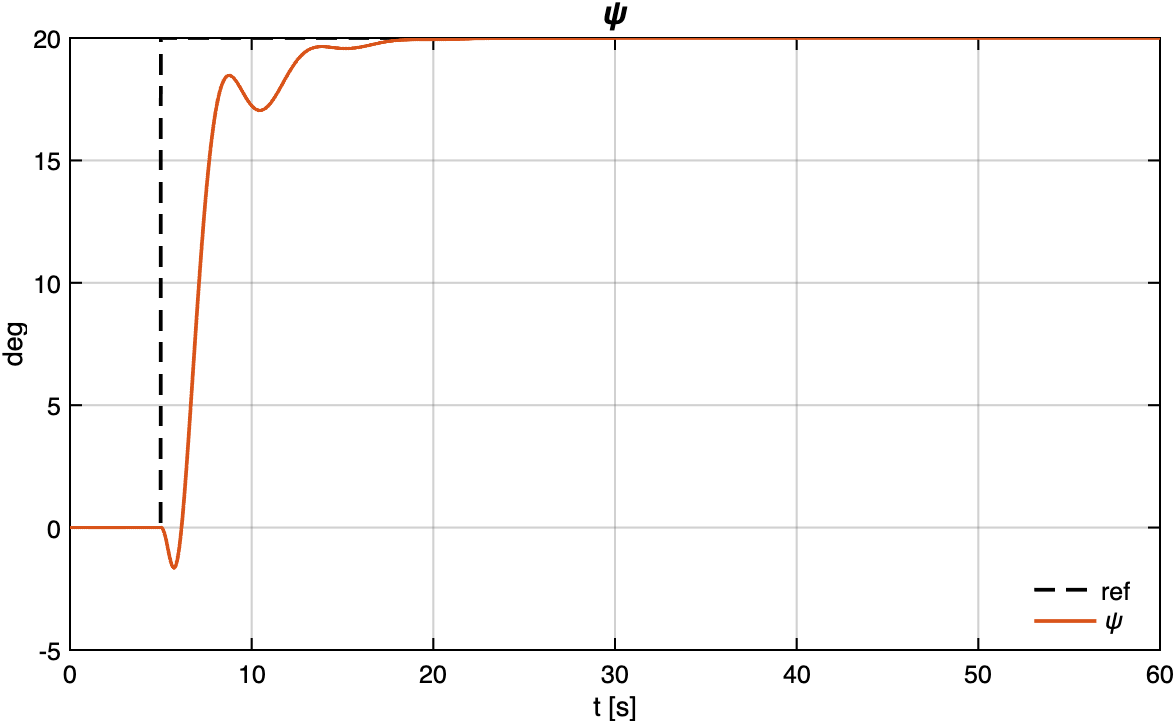
\includegraphics[width=\columnwidth]{fig_s3_hdg.png}}
\caption{Scenario 3 --- heading $\psi(t)$ tracking the $+20^\circ$ step.}
\label{fig:s3_hdg}
\end{figure}

\begin{figure}[!htbp]
\centerline{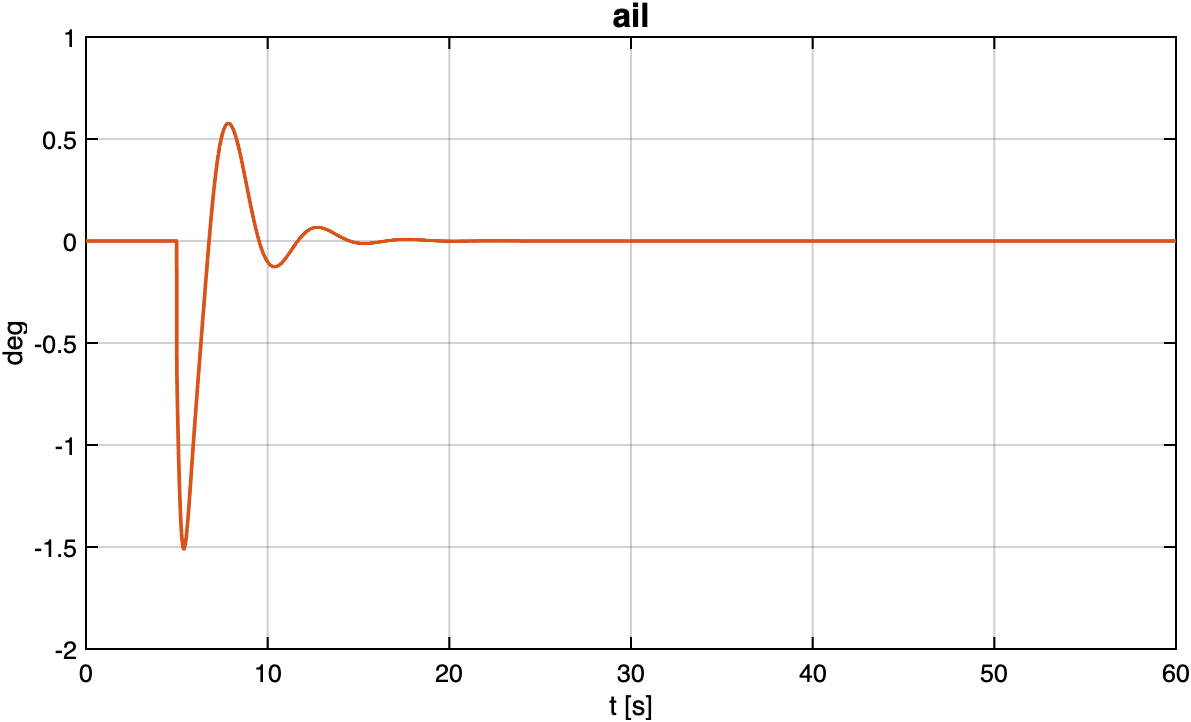
\includegraphics[width=\columnwidth]{fig_s3_ail.png}}
\caption{Scenario 3 --- aileron deflection (deg), peaking at $1.5^\circ$.}
\label{fig:s3_ail}
\end{figure}

\subsection{Scenario 4: Combined Maneuver ($+30$~m \& $+15^\circ$)}

An altitude step of $+30$~m and a heading step of $+15^\circ$ were commanded simultaneously at $t = 5$~s (Figs.~\ref{fig:s4_alt} and~\ref{fig:s4_hdg}). The elevator and aileron acted concurrently and both remained far from saturation (elevator $4.5^\circ$, aileron $1.5^\circ$, throttle $0.75$). The altitude channel reached the reference with a rise time of $8.0$~s, an overshoot of $14.4\%$, a settling time of $27.9$~s, and a steady-state error of $0.002$~m; the heading channel responded with a rise time of $1.2$~s, an overshoot of $12.8\%$, a settling time of $12.1$~s, and a negligible steady-state error.

\begin{figure}[!htbp]
\centerline{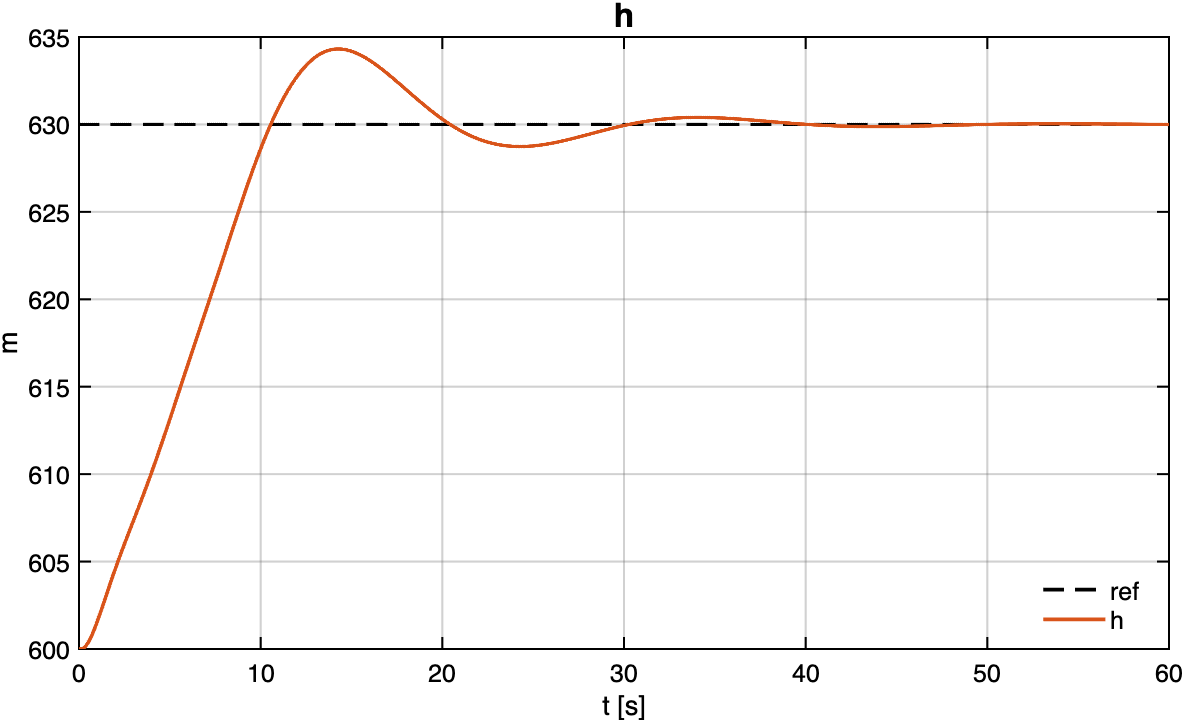
\includegraphics[width=\columnwidth]{fig_s4_alt.png}}
\caption{Scenario 4 --- altitude $h(t)$ for the simultaneous $+30$~m command.}
\label{fig:s4_alt}
\end{figure}

\begin{figure}[!htbp]
\centerline{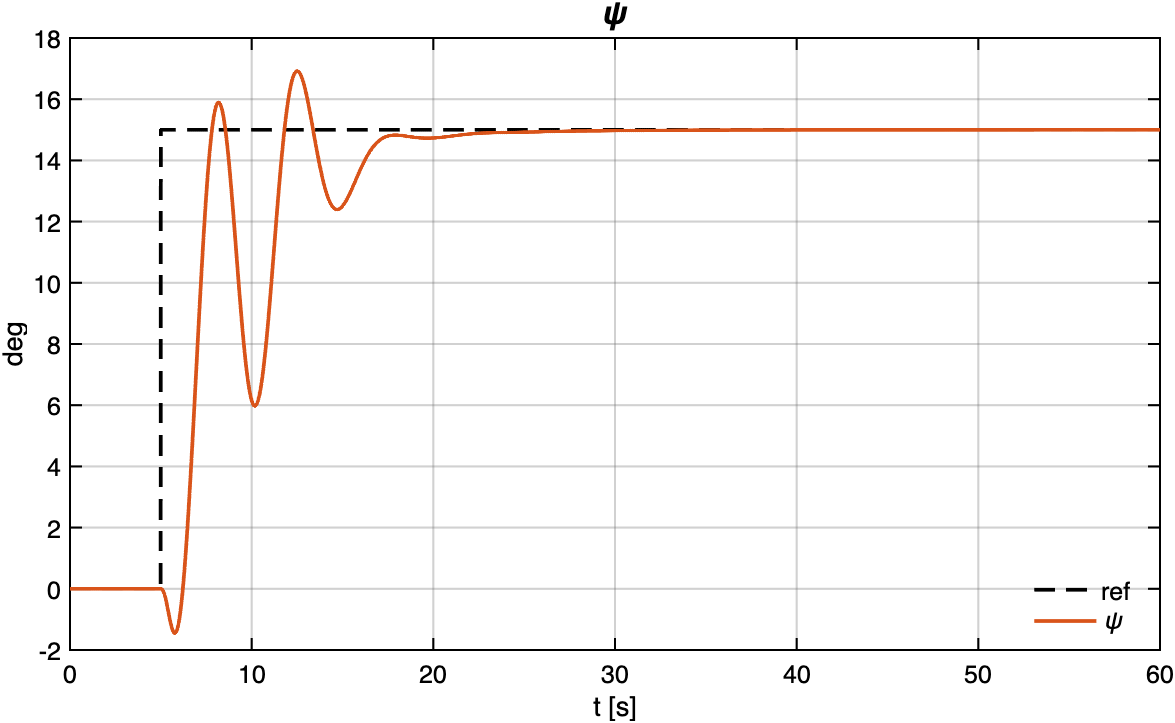
\includegraphics[width=\columnwidth]{fig_s4_hdg.png}}
\caption{Scenario 4 --- heading $\psi(t)$ for the simultaneous $+15^\circ$ command.}
\label{fig:s4_hdg}
\end{figure}

\subsection{Consolidated Performance Summary}

Table~\ref{tab:summary} consolidates the step-response indicators of every closed-loop test, together with the corresponding peak actuator demand. Across the five reference-tracking responses, the steady-state error is negligible in every loop, the overshoot never exceeds $15\%$, and the peak control-surface deflection stays at or below $4.5^\circ$ of the $\pm 25^\circ$ travel while the throttle stays at or below $0.76$ of its unit range.

\begin{table*}[!htbp]
\caption{Consolidated step-response metrics for every closed-loop test on the nonlinear plant, with the corresponding peak actuator demand.}
\label{tab:summary}
\centering
\begin{tabular}{llrrrrl}
\hline
\textbf{Scenario} & \textbf{Command} & \textbf{Rise time} & \textbf{Overshoot} & \textbf{Settling 2\%} & \textbf{SS error} & \textbf{Peak actuator} \\
\hline
Altitude hold        & $+50$~m   & $12.9$~s & $8.7\%$  & $32.7$~s & $0.04$~m  & Elevator $4.5^\circ$ \\
Velocity hold        & $+6$~m/s  & $2.5$~s  & $8.0\%$  & $8.1$~s  & $\approx 0$~m/s & Throttle $0.76$ \\
Heading hold         & $+20^\circ$ & $2.0$~s & $0.0\%$  & $10.7$~s & $\approx 0^\circ$ & Aileron $1.5^\circ$ \\
Combined --- altitude & $+30$~m   & $8.0$~s  & $14.4\%$ & $27.9$~s & $0.002$~m & Elevator $4.5^\circ$ \\
Combined --- heading  & $+15^\circ$ & $1.2$~s & $12.8\%$ & $12.1$~s & $\approx 0^\circ$ & Aileron $1.5^\circ$ \\
\hline
\end{tabular}
\end{table*}

\section{Discussion}
\label{sec:discussion}

\subsection{Summary of Main Findings}

Four observations summarize what the closed-loop campaign reveals about the cascaded PID design. First, \textit{reference tracking is achieved in every test}: all five responses reach their set-point with negligible steady-state error and overshoot below $15\%$, as the PID integrators cancel the residual offsets. Second, \textit{the behaviour matches the design intent}: the settling times follow the loop bandwidths imposed during tuning --- the slow longitudinal outer loops ($\approx 0.3$~rad/s) settle in tens of seconds, while the faster lateral loops ($\approx 0.4$~rad/s) settle in roughly $10$--$15$~s. Third, \textit{the control effort is modest and unsaturated}: the surfaces stay below $4.5^\circ$ of their $\pm 25^\circ$ range and the throttle below $0.76$, leaving an ample authority margin over the cruise envelope tested. Fourth, \textit{the decoupled cascade holds up under simultaneous excitation}: in the combined maneuver both axes track at once with only small cross-coupling (RMS deviation of the pitch reference $\approx 1^\circ$), confirming the inner-first design philosophy and the $5$--$7\times$ bandwidth separation between successive loops.

\subsection{Nonlinear Validation Insight}

A noteworthy and favourable outcome is that the response of the nonlinear plant is \emph{more} damped than that of the linear model used for design, rather than less. This is physically explainable. The quadratic aerodynamic terms --- drag growing with $V^2$ and with $\alpha^2$ --- are absent from the first-order linear model and add genuine damping to the altitude loop. In addition, the energy-to-speed coupling acts as a natural brake: pitching up to climb bleeds airspeed, which lowers the lift and curbs the climb, thereby reducing the overshoot. Crucially, the gentler response is not an artefact of actuator saturation --- the elevator peaked at only $4.5^\circ$ of its $\pm 25^\circ$ range --- nor of inconsistent initial conditions, since the fixed-trim initial state is now identical across the linear and nonlinear runs. Methodologically, this confirms that the linear model remains the right tool for control \emph{design} (\texttt{pidtune}, Bode shaping, stability margins), while the nonlinear simulation validates stability and shows that the real aircraft responds more conservatively --- not worse --- than the design model predicts.

\subsection{Comparison with Prior Work}

The results connect to the two bodies of work that frame this project. With respect to the \textit{Piper J-3 Cub 1/6 baseline} of Santos~\cite{santos2018projeto} and the open-source PIPER-1-6 toolchain~\cite{martins2025piper}, the present validation shows that the same cascaded-PID framework transfers to the hybrid VTOL airframe with only re-tuned gains. Consistently with the broader comparative analysis carried out in this project, the longitudinal (altitude and pitch) loop structure migrates directly, because the elevator effectiveness and the static pitch stability are comparable between the airframes, whereas the roll loop required re-tuning with \emph{negative} gains: the drone's aileron-control derivative is negative ($C_{l_{\delta a}} < 0$), so the sign of the roll gains must be inverted to preserve negative feedback. The remaining lateral gains were rescaled to the drone's own control effectiveness, a direct consequence of its distinct geometry and aerodynamic derivatives~\cite{saeed2018survey,theys2016influence}. With respect to the \textit{PX4 fixed-wing stack}~\cite{meier2015px4,px4dev2025}, which relies on the energy-based TECS formulation, the decoupled classical loops adopted here~\cite{stevens2016aircraft} are simpler to tune and were shown to be adequate for the cruise envelope considered, at the cost of the multivariable elegance and envelope-wide gain adaptation that TECS provides.

\subsection{Limitations of the Study}

The scope of the present validation should be read with five limitations in mind. \textit{(i) No turn coordination:} although the yaw-rate damper is active, no sideslip-feedback coordination loop ($\beta\!\to\!\delta_r$) was closed, so the heading maneuvers were run uncoordinated --- the sideslip builds up to about $4^\circ$ and the yaw rate peaks near $11^\circ$/s. \textit{(ii) Saturation untested:} all commands stayed well below the $\pm 25^\circ$ surface limits, so the large-amplitude, saturated regime was not characterized. \textit{(iii) No disturbances:} although wind and turbulence inputs exist in the model, they were not injected, so gust rejection was not assessed. \textit{(iv) Offline only:} the validation is purely simulation-based, without controller discretization or hardware-in-the-loop on the target processor. \textit{(v) Single trim point:} the gains were tuned and tested at a single cruise condition ($V_e = 12$~m/s, $h_e = 600$~m), with no gain scheduling across the flight envelope.

\subsection{Future Directions}

These limitations define the roadmap towards a flight-ready autopilot. The immediate steps are to close a sideslip-feedback turn-coordination loop ($\beta\!\to\!\delta_r$) to eliminate the adverse yaw and sideslip observed on heading captures, and to inject wind and turbulence to characterize the disturbance rejection of both axes. Beyond that, the autopilot should be exercised at the mission level with a Line-Of-Sight waypoint-guidance law, the actuators should be stressed with large-amplitude commands to characterize the saturation and anti-windup behaviour, the controller should be discretized (e.g., Tustin transform at $100$~Hz) and exercised in hardware-in-the-loop on the target microcontroller, and the design should be extended to multiple trim points with gain scheduling across the envelope. A further improvement, not yet implemented, is a feed-forward compensation of the pitch reference as a function of the commanded bank angle, $\Delta\theta_\text{ff} = f(\phi_\text{cmd})$, to anticipate the transient altitude loss that arises in banked turns (where the vertical lift component drops as $L\cos\phi$, about $13\%$ at $\phi = 30^\circ$), following the approach of Bittar~\cite{bittar2012arquitetura}.

\section{Conclusion}
\label{sec:conclusion}

This work designed and validated a classical cascaded PID autopilot for the fixed-wing cruise mode of a custom hybrid VTOL drone, leveraging the open-source PIPER-1-6 framework. The research objective was met: all longitudinal and lateral-directional loops track their references with negligible steady-state error, overshoot below $15\%$, and unsaturated control effort, including a simultaneous combined altitude-and-heading maneuver. The closed-loop validation on the nonlinear 6-DOF plant confirms the linear design and shows that the real aircraft response is, if anything, more conservative than the design model predicts. As the central contribution of this project, the Piper J-3 Cub cascaded-PID framework was shown to transfer successfully to the hybrid VTOL platform with only re-tuned gains. The overall message is that classical cascaded PID remains a robust, interpretable, and low-cost autopilot solution for this class of aircraft, and that the validated 6-DOF framework is now ready for the controller discretization, hardware-in-the-loop, and flight-test stages outlined in Section~\ref{sec:discussion}.

\section*{Acknowledgment}
The author thanks the Neusa research group at the Aeronautics Institute of Technology (ITA) for sharing the hybrid VTOL airframe and aerodynamic data, and the PIPER-1-6 project authors for providing the open-source MATLAB/Simulink toolchain on which this work is built. The Aeronautics Institute of Technology (ITA) provided the academic framework for this study.

\bibliographystyle{IEEEtran}
\bibliography{IEEEexample}

\EOD

\end{document}
